% BridgeLink ASL final project report
% ITCS 4152/5010 Introduction to Computer Vision, Spring 2026
% Compile from this directory with:
% pdflatex main.tex ; bibtex main ; pdflatex main.tex ; pdflatex main.tex

\documentclass[10pt,twocolumn,letterpaper]{article}

\usepackage[margin=0.72in]{geometry}
\usepackage{graphicx}
\usepackage{amsmath}
\usepackage{amssymb}
\usepackage{booktabs}
\usepackage{url}
\usepackage{hyperref}

\hypersetup{
    hidelinks=true
}

\setlength{\parskip}{0.35em}
\setlength{\parindent}{0pt}

\title{\vspace{-1.0em}\textbf{BridgeLink ASL: CNN vs VLM for Sign Recognition and Sentence Translation}}

\author{
Dalen Gordon \quad Ervin Gordon III \quad Frank Garcia \quad Omar Fraij\\
University of North Carolina at Charlotte\\
ITCS 4152/5010 -- Introduction to Computer Vision, Spring 2026
}

\date{}

\begin{document}
\maketitle

\begin{abstract}
BridgeLink ASL is a computer vision system for translating American Sign Language (ASL) video into English text. The project compares convolutional neural network (CNN) approaches against a vision-language model (VLM) approach across both isolated-sign recognition and sentence-level translation. The first branch is a real-time landmark CNN that converts webcam frames into MediaPipe Holistic pose and hand landmarks and classifies isolated WLASL signs from a rolling temporal buffer. The second branch is a sentence-level 3D CNN that consumes RGB How2Sign sentence clips directly, sampling 16 frames per video and learning spatiotemporal features with Conv3D layers. The third branch is a Qwen2.5-VL-3B VLM fine-tuned with QLoRA on How2Sign video-text pairs for open-ended sentence translation. The final deployed system supports live webcam recognition, uploaded word-sign clips, and uploaded sentence clips through a Gradio/Hugging Face interface with confidence-gated captions. On a 36-clip WLASL hybrid evaluation subset, the landmark CNN reaches 25.0\% top-1 accuracy and 58.3\% top-5 coverage, while a zero-shot VLM reranking workflow over the CNN top-5 reaches 25.0\% accuracy. On the repeated-sentence How2Sign subset, the strongest 3D CNN is the label-normalized top-25 model with 21 sentence classes, 335 training clips, 72 validation clips, 72 test clips, and 27.8\% held-out test accuracy. On a separate How2Sign translation experiment using 500 training clips and 100 validation clips, QLoRA fine-tuning improves the VLM from BLEU 0.13 / chrF 11.96 / ROUGE-L 0.067 to BLEU 1.26 / chrF 14.08 / ROUGE-L 0.107. Together, the experiments show that CNNs are the stronger short-phrase closed-vocabulary baseline, while the VLM better matches the full sentence translation objective even though it still needs more compute and data to become accurate.
\end{abstract}

\section{Introduction}

ASL is a complete visual language with its own grammar, facial expressions, body movement, and timing. In many everyday settings, however, hearing people do not know ASL and professional interpreters are not always available. This creates a communication barrier in classrooms, offices, medical spaces, and public services. The goal of BridgeLink ASL is to explore whether modern computer vision can reduce that barrier by converting ASL video input into readable English captions in a simple web interface.

At the beginning of the project, we treated ASL recognition as an isolated-sign classification problem using WLASL. That approach produced a practical live webcam demo because isolated words can be represented with a short temporal sequence of hand and body landmarks. Later, after instructor feedback emphasized sentence classification rather than individual signs or still images, we extended the project to How2Sign, a continuous ASL dataset whose clips correspond to full English sentence translations. That change turned the project into a more direct CNN-versus-VLM comparison: could a closed-vocabulary video classifier solve the requirement well enough, or was a video-text translation model the better direction for sentence-level ASL? This final report documents both branches and explains where each one succeeds and where it breaks down.

The project contributions are:
\begin{itemize}
    \item A working real-time ASL web application with webcam input, uploaded clip input, confidence-gated captions, and Hugging Face Space deployment support.
    \item A landmark-based temporal CNN for isolated WLASL signs using MediaPipe hand and pose landmarks.
    \item A sentence-level 3D CNN trained on RGB How2Sign full-sentence video clips, not still images.
    \item A Qwen2.5-VL-3B QLoRA fine-tuning pipeline for How2Sign video-to-English translation, preserved from the teammate Hugging Face Space workspace and imported into the main repository.
    \item Dataset analysis showing why all 31,047 local How2Sign clips cannot be used directly as independent sentence classes under a standard softmax classifier.
    \item Presentation and report figures generated with Matplotlib to show dataset sparsity, class distributions, model comparisons, 3D CNN experiments, and VLM fine-tuning results.
\end{itemize}

\section{Literature Review}

\textbf{Word-level ASL recognition.} WLASL introduced a large video benchmark for word-level ASL recognition with 2,000 glosses and standardized subset sizes such as WLASL-100 and WLASL-300 \cite{li2020wlasl}. WLASL is useful for isolated sign recognition because each clip has a single gloss label. However, it is not designed for paragraph-length translation because the labels are words, not full sentence meanings.

\textbf{Continuous ASL datasets.} How2Sign is a large-scale multimodal and multiview continuous ASL dataset with more than 80 hours of sign language videos and corresponding modalities including English transcripts, speech, depth, and pose-related data \cite{duarte2021how2sign}. The dataset is more aligned with our sentence-recognition requirement because its green-screen RGB clips are segmented around sentence-level English translations. This makes How2Sign a better fit than WLASL for testing whether a model can classify full signed sentences.

\textbf{Landmark-based models.} MediaPipe Holistic provides real-time pose, hand, and face landmark estimation on consumer hardware \cite{grishchenko2020mediapipe}. Landmark representations are compact and reduce background variation, so they are well suited for webcam demos. Skeleton and graph-based sign methods, including skeleton-aware multimodal sign recognition, also show the value of pose representations for sign understanding \cite{jiang2021slgcn}.

\textbf{3D CNN video models.} 3D CNNs extend standard 2D convolution by adding a temporal dimension. A Conv3D kernel learns local patterns across time, height, and width, making it appropriate for short video clips where motion matters \cite{tran2015c3d}. For our sentence branch, the 3D CNN receives sampled RGB frame volumes and learns from motion and appearance jointly.

\textbf{Transformer and VLM baselines.} Sign Language Transformers frame sign recognition as a sequence modeling task \cite{camgoz2020signtransformer}. Beyond pure classifiers, recent vision-language models can directly map video content into text. Parameter-efficient fine-tuning methods such as LoRA \cite{hu2022lora} and QLoRA \cite{dettmers2023qlora} make this practical on smaller hardware by training lightweight adapters instead of fully updating every model weight. In our project, this became the main sentence-translation alternative to the CNN approach.

\section{Data Description}

Following the dataset-reporting style used in Section 3 of the Toyota Smarthome Untrimmed paper \cite{dai2020toyota}, we describe the source, modalities, labels, splits, and limitations of each dataset used in BridgeLink ASL.

\subsection{WLASL Word-Level Data}

WLASL is a public word-level ASL video dataset where each clip is labeled by an English gloss, such as \texttt{help}, \texttt{drink}, or \texttt{yes}. In our project, WLASL supports the live webcam and uploaded isolated-sign tab. The deployed WLASL label map contains 100 word classes. The reported WLASL evaluation artifact is a 36-clip WLASL-25 hybrid subset with 22 true classes. Each record contains the ground-truth label and the CNN top-5 candidates used for the VLM comparison.

The WLASL branch does not solve full sentence translation. It is useful because it demonstrates real-time sign recognition and produces sensible output from webcam input, but it remains an isolated-sign classifier.

\subsection{How2Sign Sentence Data}

How2Sign provides continuous ASL videos aligned with English sentence translations. The data used in this project are green-screen RGB frontal-view clips. Each clip shows a signer from the upper body view, including the hands, arms, torso, face region, and green-screen background. The label is an English sentence string, for example \texttt{Thank you.}, \texttt{Here we go.}, or \texttt{One, two, three.}

Our local How2Sign processing pipeline matched 31,047 sentence clips from the available RGB clip and translation files. However, approximately 30,008 of those labels are unique sentence strings. This is the central data issue. A standard softmax classifier needs multiple examples of each class so it can learn what visual variation belongs to the same label. If nearly every sentence appears once, then treating all 31,047 clips as 31,047 classes becomes memorization rather than learnable supervised classification.

To make the task trainable within the current 3D CNN structure, we selected repeated sentence labels. Table~\ref{tab:how2sign-subsets} summarizes the usable repeated subsets. The final model uses the top-25 repeated sentence subset after conservative label normalization. Normalization merges punctuation and spelling variants such as \texttt{Hi!} with \texttt{Hi.}, \texttt{O.k.} with \texttt{Okay.}, and \texttt{Alright.} with \texttt{All right.} This reduced the top-25 subset from 25 raw labels to 21 normalized labels while keeping the same 479 clips.

For the VLM branch, the data are represented differently. Instead of treating each sentence as a class, the imported Qwen2.5-VL workspace uses JSONL rows with \texttt{id}, \texttt{video\_path}, and \texttt{translation}. This means the model can train on arbitrary sentence-video pairs even if every sentence string is unique. The archived experiment we imported into the main repository uses 500 How2Sign training clips and 100 validation clips. This is a much smaller slice of the full dataset than the 31k local clip inventory, but unlike the 3D CNN classifier, the VLM objective is compatible with open-ended sentence labels.

\begin{table}[t]
\centering
\small
\begin{tabular}{lrr}
\toprule
Subset & Clips & Classes \\
\midrule
All matched How2Sign clips & 31,047 & 30,008 \\
Repeated at least 2 times & 1,487 & 448 \\
Repeated at least 3 times & 769 & 89 \\
Repeated at least 5 times & 611 & 41 \\
Repeated at least 8 times & 531 & 26 \\
Top-12 repeated subset & 218 & 12 \\
Top-25 repeated subset & 479 & 25 \\
Top-25 normalized subset & 479 & 21 \\
\bottomrule
\end{tabular}
\caption{How2Sign sentence-label sparsity. Most full sentence labels occur once, so the supervised CNN was trained on repeated sentence subsets.}
\label{tab:how2sign-subsets}
\end{table}

\begin{figure}[t]
\centering

\includegraphics[width=\linewidth]{figures/how2sign_dataset_constraint.png}
\caption{How2Sign dataset constraint. The project has access to many sentence clips, but most labels are singletons, which limits ordinary closed-vocabulary classification.}
\label{fig:dataset-constraint}
\end{figure}

\begin{figure}[t]
\centering

\includegraphics[width=\linewidth]{figures/how2sign_top25_class_distribution.png}
\caption{Class distribution for the normalized top-25 How2Sign sentence subset used by the final 3D CNN.}
\label{fig:class-distribution}
\end{figure}

\section{Method}

\subsection{System Pipeline}

BridgeLink ASL is implemented as a Gradio application. The live tab accepts webcam frames, the word clip tab accepts uploaded or recorded WLASL-style clips, and the sentence tab accepts uploaded How2Sign-style RGB sentence clips. The output is a caption area designed to avoid showing uncertain answers. When confidence is below the display threshold, the interface shows that no confident sign or sentence has been produced yet.

\subsection{Landmark CNN for Word-Level Recognition}

The WLASL branch uses MediaPipe Holistic as a fixed feature extractor. For each sampled frame, we collect 21 left-hand landmarks, 21 right-hand landmarks, and 33 pose landmarks. Each landmark contributes $(x,y,z)$ coordinates, producing a 225-dimensional feature vector per frame. A clip is represented as a sequence of 32 frames, so the input tensor is $32 \times 225$.

The landmark classifier is a temporal 1D CNN:
\begin{itemize}
    \item Input: 32-frame landmark sequence with 225 features per frame.
    \item Layers: BatchNorm1D, Conv1D with 128 channels, BatchNorm, ReLU, Dropout, Conv1D with 128 channels, BatchNorm, ReLU, MaxPool1D, Conv1D with 256 channels, BatchNorm, ReLU, Dropout, AdaptiveAvgPool1D, and a final linear classifier.
    \item Output: softmax probabilities over the deployed word-label set.
    \item Runtime filter: predictions are only displayed after confidence and stability checks so captions do not flicker.
\end{itemize}

The training notebook optimizes cross entropy with label smoothing 0.1 using AdamW, learning rate $10^{-3}$, weight decay $10^{-2}$, batch size 64, 50 epochs, and cosine annealing. The purpose of this model is to provide a fast, stable, real-time baseline for the live demo, not to solve sentence-level ASL.

\subsection{Sentence-Level 3D CNN}

The sentence model is the main video CNN contribution. It reads RGB video frames directly rather than landmarks. Each sentence clip is decoded, uniformly sampled to 16 frames, resized to $112 \times 112$, and stacked into a 5D input tensor:
\[
\mathbf{X} \in \mathbb{R}^{16 \times 112 \times 112 \times 3}.
\]

The final 3D CNN architecture is:
\begin{itemize}
    \item Input layer named \texttt{clip\_frames}.
    \item Rescaling layer dividing pixels by 255.
    \item Conv3D block 1: 16 filters, $3 \times 3 \times 3$ kernel, ReLU, same padding, BatchNorm, MaxPool3D with pool $(1,2,2)$.
    \item Conv3D block 2: 32 filters, $3 \times 3 \times 3$ kernel, ReLU, same padding, BatchNorm, MaxPool3D with pool $(2,2,2)$.
    \item Conv3D block 3: 64 filters, $3 \times 3 \times 3$ kernel, ReLU, same padding, BatchNorm, MaxPool3D with pool $(2,2,2)$.
    \item GlobalAveragePooling3D layer named \texttt{clip\_embedding}.
    \item Dropout with rate 0.4.
    \item Dense softmax classifier over the sentence classes.
\end{itemize}

The cost function is sparse categorical cross entropy:
\[
\mathcal{L} = -\frac{1}{N}\sum_{i=1}^{N}\log p_\theta(y_i \mid \mathbf{X}_i),
\]
where $\mathbf{X}_i$ is the sampled RGB clip volume and $y_i$ is the sentence-class index. The optimizer is Adam \cite{kingma2015adam} with learning rate $3 \times 10^{-4}$. We used batch size 2 because raw RGB clip volumes are memory-heavy compared with landmark tensors. The default training schedule is 20 epochs with model checkpointing on validation accuracy, early stopping patience 5, and ReduceLROnPlateau on validation loss with patience 2 and factor 0.5.

\subsection{Qwen2.5-VL VLM Translation Path}

The teammate VLM workspace, originally maintained as a Hugging Face Space repository and then imported into the main project repository, fine-tunes \texttt{Qwen/Qwen2.5-VL-3B-Instruct} on How2Sign sentence-video pairs. This branch treats the task as conditional generation rather than classification. Given a video and a prompt, the model autoregressively generates the target English translation.

The prompt used during training and evaluation is:
\begin{quote}
\small
Translate the American Sign Language video into natural English. Output only the English translation.
\end{quote}

The video preprocessing settings match the lightweight 3D CNN clip budget closely enough to support a fair engineering comparison:
\begin{itemize}
    \item Sampling rate: 2 FPS.
    \item Maximum frames: 16.
    \item Maximum decoded output length: 96 new tokens.
    \item Deterministic generation: no sampling, temperature 0.0.
\end{itemize}

Fine-tuning uses LoRA adapters with a QLoRA setup \cite{hu2022lora,dettmers2023qlora}. The archived configuration trains for 1 epoch with per-device batch size 1, gradient accumulation 8, learning rate $10^{-4}$, LoRA rank 16, LoRA alpha 32, LoRA dropout 0.05, NF4 4-bit quantization, and gradient checkpointing. The trainable target modules are the attention and MLP projection layers:
\texttt{q\_proj}, \texttt{k\_proj}, \texttt{v\_proj}, \texttt{o\_proj}, \texttt{gate\_proj}, \texttt{up\_proj}, and \texttt{down\_proj}.

The training loss for this branch is token-level autoregressive cross entropy over the reference translation text, with prompt tokens masked so only the target translation contributes to the loss. This is the key conceptual difference from the CNN branch: the VLM does not require a fixed sentence class list and is therefore compatible with unique sentence labels.

\subsection{Embedding Retrieval Mode}

The Hugging Face sentence demo can load the trained 3D CNN and use the \texttt{clip\_embedding} layer as a video embedding. At inference time, the uploaded clip is embedded and compared against a small support index built from repeated training clips. This nearest-neighbor mode is useful for the demo because it often gives more stable matches for short repeated phrases than raw softmax confidence alone. The report metrics, however, still evaluate the supervised 3D CNN classification checkpoints on held-out splits.

\section{Experimentation}

\subsection{Implementation}

The project is implemented in Python 3.11. The live application uses Gradio, OpenCV, MediaPipe, PyTorch, TensorFlow/Keras, NumPy, and Hugging Face Hub. The sentence CNN is trained through the command-line module \texttt{bridgelink\_asl.cli.train\_cnn\_model}. The VLM experiment uses a separate Qwen2.5-VL workspace with \texttt{transformers}, \texttt{accelerate}, \texttt{peft}, \texttt{bitsandbytes}, \texttt{decord}, \texttt{datasets}, \texttt{evaluate}, \texttt{sacrebleu}, and \texttt{rouge-score}. That workspace was imported from the teammate Hugging Face Space into the main repository under \texttt{vlm\_hf\_space/} so the final GitLab submission contains the full VLM code and archived outputs. Figures are generated with Matplotlib from saved metrics and dataset summaries.

\subsection{Splits}

The final How2Sign normalized sentence dataset contains 479 clips across 21 normalized sentence labels. The split used for the final 3D CNN is:
\begin{itemize}
    \item Training: 335 clips.
    \item Validation: 72 clips.
    \item Test: 72 clips.
\end{itemize}

The WLASL hybrid evaluation subset contains 36 test clips across 22 true labels. It is used to evaluate the landmark CNN and VLM reranking workflow.

The imported How2Sign VLM experiment uses prepared JSONL manifests with:
\begin{itemize}
    \item Training: 500 sampled sentence-video pairs.
    \item Validation / evaluation: 100 sampled sentence-video pairs.
\end{itemize}
These clips come from the broader How2Sign sentence corpus and are evaluated with translation metrics rather than classification accuracy.

\subsection{Model Variants}

We ran several CNN and VLM experiments:
\begin{itemize}
    \item \textbf{Top-12 repeated subset:} early feasibility test with 218 clips and 12 classes.
    \item \textbf{Top-25 raw subset:} larger closed vocabulary with 479 clips and 25 sentence labels.
    \item \textbf{Top-25 normalized subset:} duplicate-label merge that reduces the label space to 21 classes.
    \item \textbf{Continued training:} additional epochs from the top-25 checkpoint.
    \item \textbf{Class weighting:} balanced class weights to compensate for label imbalance.
    \item \textbf{How2Sign VLM baseline:} zero-shot Qwen2.5-VL-3B evaluation on 100 validation clips.
    \item \textbf{How2Sign VLM QLoRA fine-tune:} 1 epoch of adapter training on 500 training clips, evaluated on the same 100 validation clips.
\end{itemize}

\section{Results}

\subsection{Working Model Output}

The final application produces sensible output in three ways. The live webcam tab displays stabilized word predictions from the landmark CNN. The upload tab returns word-level predictions with confidence values. The How2Sign sentence tab returns a sentence-level best match from the 3D CNN sentence model or withholds the caption if the result is not confident enough. This satisfies the modeling requirement that the system accepts input and produces interpretable output.

\subsection{Quantitative Results}

Table~\ref{tab:overall-results} gives the classification-side evaluation results. The best 3D CNN is the normalized How2Sign top-25 model. Its accuracy is not high in an absolute sense, but it is better than the raw top-25 and top-12 sentence baselines and is trained on full sentence video clips. The VLM results are reported separately because they are translation metrics rather than class-accuracy metrics.

\begin{table}[t]
\centering
\small
\resizebox{\linewidth}{!}{%
\begin{tabular}{lrrrr}
\toprule
Model / Track & Eval clips & Classes & Accuracy & Macro F1 \\
\midrule
WLASL landmark CNN top-1 & 36 & 22 true & 25.0\% & 15.1\% \\
WLASL VLM rerank & 36 & 22 true & 25.0\% & -- \\
How2Sign 3D CNN normalized & 72 & 21 & 27.8\% & 6.0\% \\
\bottomrule
\end{tabular}
}
\caption{Primary classification results. The WLASL branch is word-level; the How2Sign branch is sentence-level RGB video classification.}
\label{tab:overall-results}
\end{table}

\begin{table}[t]
\centering
\small
\resizebox{\linewidth}{!}{%
\begin{tabular}{lrrrrr}
\toprule
How2Sign experiment & Classes & Train & Val & Test & Test acc. \\
\midrule
Top-12 repeated & 12 & 150 & 34 & 34 & 14.7\% \\
Top-25 raw & 25 & 335 & 72 & 72 & 20.8\% \\
Top-25 normalized & 21 & 335 & 72 & 72 & \textbf{27.8\%} \\
Top-25 continued & 25 & 335 & 72 & 72 & 18.1\% \\
Top-25 weighted & 25 & 335 & 72 & 72 & 13.9\% \\
\bottomrule
\end{tabular}
}
\caption{Sentence-level 3D CNN ablation results. Label normalization gave the strongest held-out test accuracy.}
\label{tab:how2sign-results}
\end{table}

\begin{table}[t]
\centering
\small
\resizebox{\linewidth}{!}{%
\begin{tabular}{lrrrr}
\toprule
How2Sign VLM run & Samples & BLEU & chrF & ROUGE-L \\
\midrule
Base Qwen2.5-VL-3B & 100 & 0.13 & 11.96 & 0.0668 \\
QLoRA fine-tuned & 100 & \textbf{1.26} & \textbf{14.08} & \textbf{0.1074} \\
\bottomrule
\end{tabular}
}
\caption{How2Sign VLM translation results from the imported teammate workspace. Fine-tuning improves every reported translation metric, although the absolute scores remain low.}
\label{tab:vlm-results}
\end{table}

\begin{figure}[t]
\centering

\includegraphics[width=\linewidth]{figures/how2sign_subset_benchmark.png}
\caption{Top-12, top-25, and normalized top-25 3D CNN benchmark comparison.}
\label{fig:subset-benchmark}
\end{figure}

\begin{figure}[t]
\centering

\includegraphics[width=\linewidth]{figures/how2sign_top25_experiment_comparison.png}
\caption{3D CNN experiment comparison. The normalized sentence labels produced the best test accuracy.}
\label{fig:experiment-comparison}
\end{figure}

\begin{figure}[t]
\centering
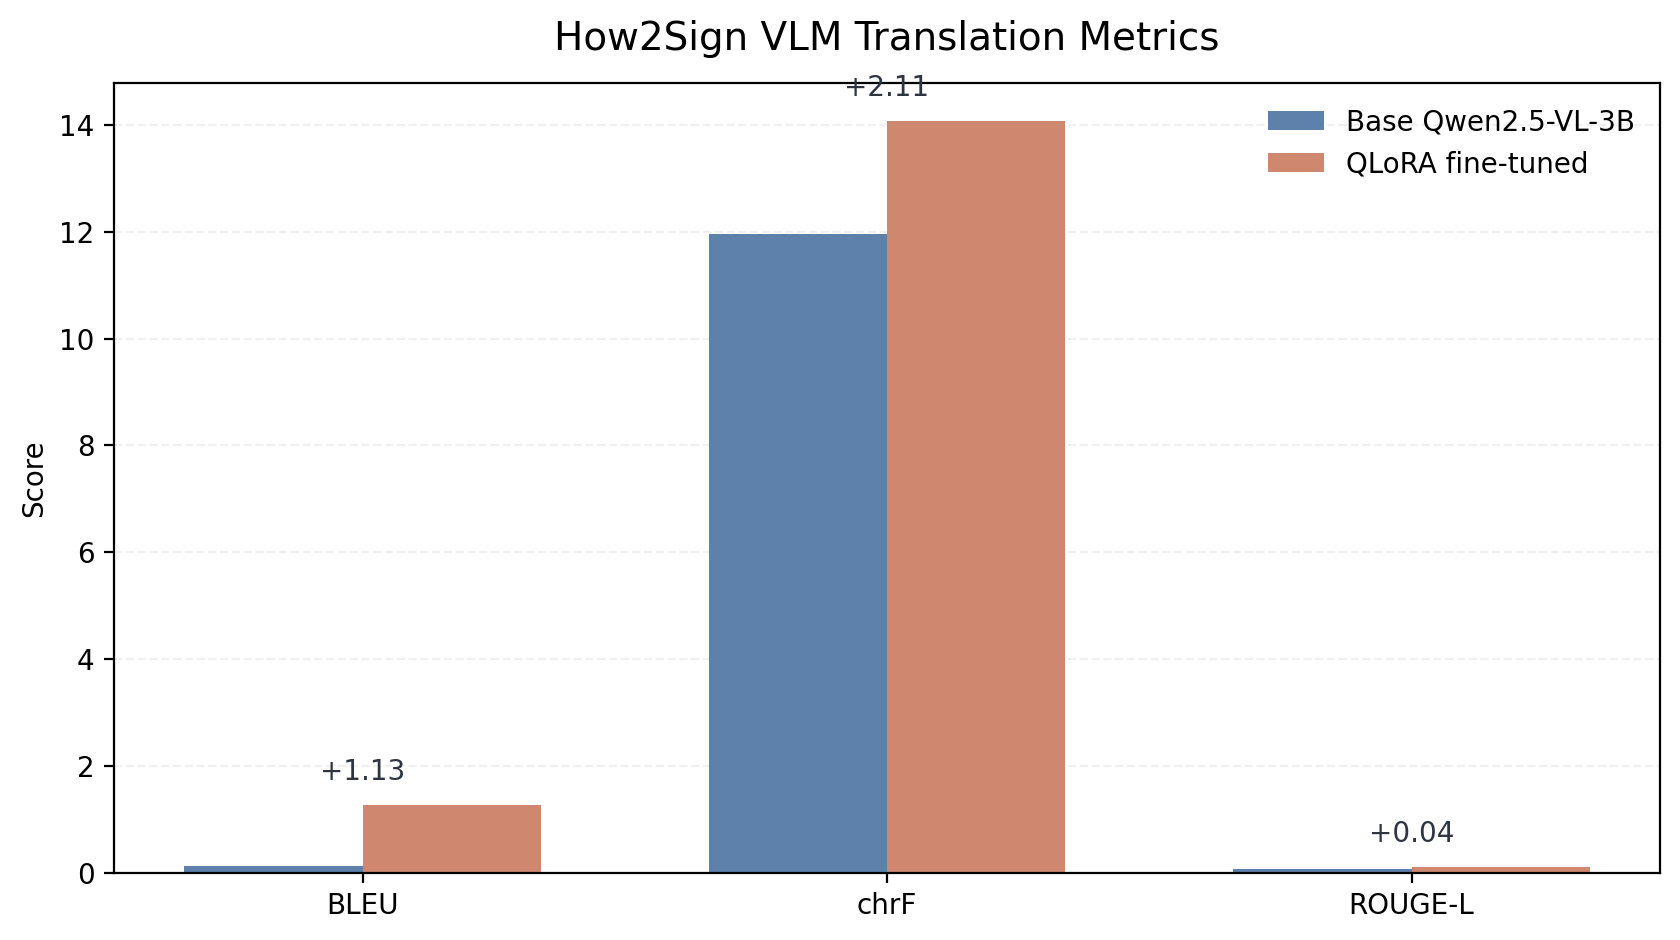
\includegraphics[width=\linewidth]{figures/vlm_how2sign_metrics.png}
\caption{How2Sign VLM baseline versus QLoRA fine-tuned translation metrics on the archived 100-sample validation evaluation.}
\label{fig:vlm-metrics}
\end{figure}

\subsection{Observations}

The most important result is that dataset structure matters more than raw storage size. The project has access to about 31,000 local How2Sign clips, but a closed-vocabulary sentence classifier cannot learn 30,000 classes with one example per class. The repeated-sentence subset is much smaller, but it provides a trainable objective because each class has multiple examples.

Label normalization improved the sentence model because the original labels contained separate classes for sentence variants that are visually and semantically almost identical. For example, \texttt{Okay.}, \texttt{Okay?}, and \texttt{O.k.} should not be treated as unrelated classes. Merging these labels reduced unnecessary class fragmentation and improved test accuracy from 20.8\% to 27.8\%.

The imported VLM experiment shows the opposite tradeoff. Because the VLM predicts open-ended text, it can be trained on sentence-video pairs without repeated class labels. This makes it the more principled approach for full paragraph-level or free-form sentence translation. However, the archived fine-tuning run is still compute-limited and data-limited: it uses only 500 training clips and 100 evaluation clips, and the resulting BLEU / chrF / ROUGE-L scores remain low even though they improve over the base model. Qualitative predictions reveal another challenge: the model often produces generic instructional language or safety-style refusal text instead of grounded translations.

Class weighting and continued training did not improve the final 3D CNN result. This suggests the bottleneck is not simply undertraining. The harder problem is limited repeated sentence data, visual similarity between short phrases, and the fact that English sentence labels do not always align perfectly with ASL timing. In short, the CNN is the stronger short-phrase closed-vocabulary baseline, while the VLM is the architecture that scales more naturally to unrestricted sentence translation.

\subsection{Qualitative Results and Demo}

The live demo is intentionally confidence-gated. If the model does not meet the confidence threshold, the UI displays ``No Confident Sign Yet'' or ``No Confident Sentence Yet'' rather than showing a likely incorrect caption. This is important for accessibility because a wrong caption can be worse than no caption. In successful sentence demos, short repeated phrases such as \texttt{Thank you.}, \texttt{One, two, three.}, and \texttt{Here we go.} are the best candidates because they exist in the repeated How2Sign training subset.

The VLM branch is more useful as an offline experiment than as the final live demo path. In the archived predictions, the fine-tuned model does move away from outright refusals and toward sentence-like English outputs, but many generations are still semantically generic rather than clip-specific. That makes the VLM promising as the long-term direction, but not yet reliable enough to replace the gated CNN demo in a classroom presentation.

\section{Limitations and Future Work}

The current 3D CNN satisfies the requirement of using video clips of full ASL sentences, but it is a closed-vocabulary sentence classifier. It cannot read arbitrary paragraphs of sign language. To use all 31,047 clips effectively, the training objective would need to change from sentence-class classification to a video-to-text or contrastive video-text objective. The VLM branch already moves in that direction, but the current QLoRA run is too small to be competitive yet.

Accuracy could be improved by:
\begin{itemize}
    \item Expanding the repeated-label subset with more clips per sentence class for the CNN branch.
    \item Using signer-aware or source-aware train/test splits when signer metadata is available.
    \item Fine-tuning a pretrained video backbone instead of training a small 3D CNN from scratch.
    \item Combining RGB frames with landmark or pose streams to reduce background and clothing sensitivity.
    \item Training the VLM on a much larger portion of How2Sign instead of the current 500/100 sample budget.
    \item Evaluating with additional translation metrics and human judgment to better judge semantic correctness.
    \item Training a retrieval model that uses sentence text embeddings instead of requiring every sentence to be a separate class.
\end{itemize}

\section{Conclusion}

BridgeLink ASL demonstrates a complete CNN-versus-VLM project pipeline for ASL recognition and translation. The landmark CNN provides a practical real-time word-sign demo, the How2Sign 3D CNN provides a working full-sentence video classifier, and the imported Qwen2.5-VL workspace provides the open-ended translation branch that better matches long-form sentence understanding. The best 3D CNN reaches 27.8\% test accuracy on a 21-class repeated-sentence task, while the fine-tuned VLM improves over its base checkpoint on BLEU, chrF, and ROUGE-L but still needs more training scale. The project therefore meets the core technical requirements while also making an honest technical point: CNNs are currently the stronger constrained demo path, but VLM-style video-to-text modeling is the more scalable direction for true sentence and paragraph translation.

\section*{Acknowledgments}

We thank the creators of WLASL, How2Sign, MediaPipe, TensorFlow, PyTorch, Gradio, and Hugging Face for releasing tools and datasets that made this project possible.

{\small
\bibliographystyle{plain}
\bibliography{references}
}

\end{document}
